\documentclass[handout]{beamer}
\usetheme{metropolis}

\usepackage{microtype}
\usepackage{changepage}
\usepackage{graphicx}
\usepackage{wrapfig}
\usepackage{tikz}
\usetikzlibrary{calc}  % Add calc library for better TikZ control
\usepackage{subcaption} % For side-by-side figures with captions


\theoremstyle{definition}
\newtheorem{noitalicstheorem}{Theorem}

\DeclareMathOperator{\GL}{GL}
\DeclareMathOperator{\M}{M}

\newcommand{\C}{k}
\renewcommand{\O}{\mathcal{O}}
\newcommand{\Q}{\mathbb{Q}}
\newcommand{\Z}{\mathbb{Z}}
\newcommand{\p}{\mathfrak{p}}

\usetheme{metropolis}
\definecolor{mynavy}{RGB}{35, 55, 59}
\definecolor{myorange}{RGB}{235, 129, 27}
\definecolor{myteal}{RGB}{92, 188, 172}
\definecolor{mygreen}{RGB}{11, 176, 161}
\definecolor{myblue}{RGB}{130, 158, 117}
\metroset{block=fill}

%\setbeamercolor{block body}{bg=transparent}
%\setbeamercolor{block title}{bg=transparent}

\theoremstyle{definition}
\newtheorem{singularitiestheorem}{Theorem (Cones detect singularities)}
\newtheorem{proposition}{Proposition}


\title{Toric Varieties}
%\subtitle{Three perspectives}
\author{Declan Fletcher}
\date{October 2024}

\begin{document}
\begin{frame}
\titlepage
\end{frame}

\begin{frame}
\frametitle{What are toric varieties, and why study them?}
\pause
Algebraic varieties are geometric spaces defined by solutions to \alert{polynomial equations}.

\pause
In general, these are complicated and difficult to study.

\pause
\alert{Toric varieties} are a special class of varieties determined by a \alert{convex cone}.
\end{frame}

\begin{frame}
\frametitle{Algebraic varieties}
\centering
\begin{minipage}[t]{0.49\textwidth}
\centering
\begin{figure}
\begin{tikzpicture}
  \draw[ultra thick, myorange, samples=100, smooth] 
    plot[domain=0:360] ({cos(\x)}, {sin(\x)});
\end{tikzpicture}
\vspace{0.05cm}
\caption*{$x^2+y^2=1$}
\end{figure}
\end{minipage}
\hfill
\begin{minipage}[t]{0.49\textwidth}
    \centering
\vspace{-1cm}
\begin{figure}
    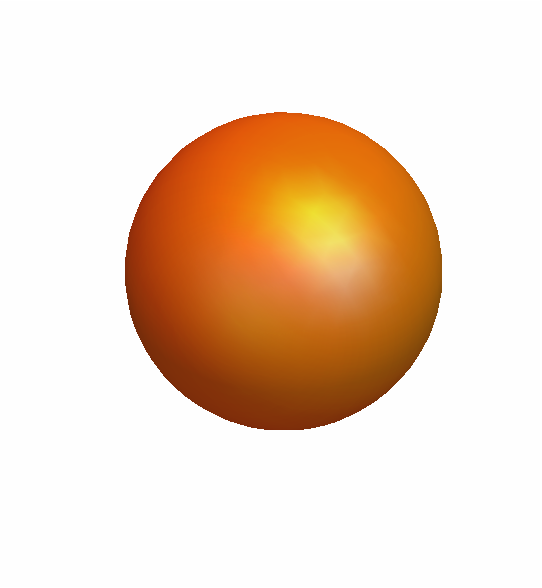
\includegraphics[width=0.75\linewidth]{orange_sphere}
	\vspace{-1.2cm}
     \caption*{$x^2+y^2+z^2=1$}
\end{figure}
\end{minipage}
%\vfill
\begin{minipage}[t]{0.49\textwidth}
    \centering
\vspace{-0cm}
\begin{figure}
\begin{tikzpicture}
  \draw[ultra thick, myorange, samples=100, smooth, domain=-2:0.95, variable=\x] 
    plot ({\x}, {sqrt((\x)^3 + 2*(\x)^2)});
  \draw[ultra thick, myorange, samples=100, smooth, domain=-2:0.95, variable=\x] 
    plot ({\x}, {-sqrt((\x)^3 + 2*(\x)^2)});
\end{tikzpicture}
\caption*{$y^2=x^3+2x^2$}
\end{figure}
\end{minipage}
\hfill
\begin{minipage}[t]{0.49\textwidth}
    \centering
\vspace{-0.2cm}
\begin{figure}
    
\includegraphics[width=0.7\linewidth]{orange_cone}
	\vspace{-.25cm}
    \caption*{$xy=z^2$}
\end{figure}
\end{minipage}
\end{frame}

\begin{frame}[t]
\frametitle{The definition of a variety}
\onslide<1->{
Varieties are sets of solutions $(a_1, \ldots, a_n) \in \mathbb{C}^n$ to poly.\ equations
$$f_1(a_1, \ldots, a_n) = 0, \quad \ldots, \quad f_s(a_1, \ldots, a_n) = 0.$$
}

\vspace{-0.2cm}

\begin{minipage}{0.45\textwidth}
\linespread{0.2}\selectfont  % Adjust the line spacing inside the minipage
\onslide<2->{Choose the zero polynomial:
$$\rightsquigarrow \mathbb{C}^n.$$}
\onslide<3->{\noindent Choose $y^2 = x^3 + 2x^2$:
$$\rightsquigarrow \text{\textcolor{blue}{singular curve}.}$$}
\onslide<4->{\noindent Choose $xy = 1$:
$$\rightsquigarrow \{(t, t^{-1}) : t \in \mathbb{C}^\times\} \cong \mathbb{C}^\times.$$}
\end{minipage}
\hfill
\begin{minipage}{0.45\textwidth}
\onslide<3->{
\begin{tikzpicture}
  % Draw axes
  \draw[->] (-2.7, 0) -- (2.2, 0); % node[right] {$x$};
  \draw[->] (0, -2) -- (0, 2); % node[above] {$y$};

  % Plot the curve y^2 = x^3 - x + 1 manually
  \draw[thick, blue, samples=100, smooth, domain=-2:1.1, variable=\x] 
    plot ({\x}, {sqrt((\x)^3 + 2*(\x)^2)});
  \draw[thick, blue, samples=100, smooth, domain=-2:1.1, variable=\x] 
    plot ({\x}, {-sqrt((\x)^3 + 2*(\x)^2)});
\end{tikzpicture}
}
\end{minipage}

\onslide<4->{
$\mathbb{C}^\times$ is called an algebraic \alert{torus}. The $d$-dimensional torus is $(\mathbb{C}^\times)^d$.
}
\end{frame}

\begin{frame}
\frametitle{Convex cones}
To understand toric varieties, we need to understand convex cones.

\pause
We consider \alert{polyhedral cones}. These are sets in $\mathbb{R}^n$ of the form
$$\sigma = \mathrm{span}_{\mathbb{R}_{\ge 0}}\{v_1, \ldots, v_r\},$$
for some $v_1, \ldots, v_r \in \mathbb{R}^n$.
$\sigma$ is \alert{rational} if we can take each $v_i \in \mathbb{Z}^n$.

\pause
\begin{minipage}[t]{0.49\textwidth}
\centering
\begin{figure}
\begin{tikzpicture}
            \fill[gray!30] (0,0) -- (-1.1,1.1) -- (-1.1,1.6) -- (1.1,1.6) -- (1.1, 1.1) -- cycle;
            
            % Axes
            \draw[->] (-1.25,0) -- (1.25,0);
            \draw[->] (0,-0.75) -- (0,1.75);
            
            % Lattice points
            \foreach \x in {-1,-0.5,0,0.5,1,}
                \foreach \y in {-0.5,0,0.5,1,1.5}
                    \fill (\x,\y) circle (1pt);

            % Vectors
            \draw[->, ultra thick] (0,0) -- (-0.5,0.5);
            \draw[->, ultra thick] (0,0) -- (0.5,0.5);
            \node at (0.75, 1.25) {$\sigma$};
\end{tikzpicture}
\end{figure}
\end{minipage}
\hfill
\begin{minipage}[t]{0.49\textwidth}
    \centering
\begin{figure}
\begin{tikzpicture}
            \fill[gray!30] (0,0) -- (-0.8,1.6) -- (1.1,1.6) -- (1.1,0) -- cycle;
            
            % Axes
            \draw[->] (-1.25,0) -- (1.25,0);
            \draw[->] (0,-0.75) -- (0,1.75);
            
            % Lattice points
            \foreach \x in {-1,-0.5,0,0.5,1,}
                \foreach \y in {-0.5,0,0.5,1,1.5}
                    \fill (\x,\y) circle (1pt);

            % Vectors
            \draw[->, ultra thick] (0,0) -- (0.5,0);
            \draw[->, ultra thick] (0,0) -- (-0.5,1);
            \node at (0.75, 1.25) {$\sigma$};
\end{tikzpicture}
\end{figure}
\end{minipage}

\end{frame}


\begin{frame}
\frametitle{Dual cones}
\textbf{Fix}: cone $\sigma$.
\pause
The \alert{dual cone} is the set of linear functionals which are non-negative on $\sigma$:
$$\sigma^\vee := \{u \in (\mathbb{R}^n)^* : u(v) \ge 0 \text{ for all } v \in \sigma\}.$$
\begin{figure}[H]
    \centering
    \begin{tikzpicture}[scale=1.2]
        % Left diagram
        \begin{scope}[shift={(-2,0)}]
            % Shaded area
            \fill[gray!30] (0,0) -- (-1.05, 2.1) -- (2.1,2.1) -- (2.1,0) -- cycle;
            
            % Axes
            \draw[->] (-1.25,0) -- (2.25,0);
            \draw[->] (0,-0.25) -- (0,2.25);
            
            % Lattice points
            \foreach \x in {-1,-0.5,0,0.5,1,1.5,2}
                \foreach \y in {0,0.5,1,1.5,2}
                    \fill (\x,\y) circle (1pt);

            % Vectors
            \draw[->, ultra thick] (0,0) -- (0.5,0);
            \draw[->, ultra thick] (0,0) -- (-0.5,1);
            \node at (1.75, 1.75) {$\sigma$};
        \end{scope}

        % Right diagram
        \begin{scope}[shift={(2,0)}]
            % Shaded area
            \fill[gray!30] (0,0) -- (0,2.1) -- (2.1,2.1) -- (2.1, 1.05) -- cycle;
            
            % Axes
            \draw[->] (-1.25,0) -- (2.25,0);
            \draw[->] (0,-0.25) -- (0,2.25);
            
            % Lattice points
            \foreach \x in {-1,-0.5,0,0.5,1,1.5,2}
                \foreach \y in {0,0.5,1,1.5,2} {
                    \fill (\x,\y) circle (1pt);
                }
                
%			  % Labels
%			  \node[anchor=south west] at (0, 0) {\!\!\! \tiny \alert{$1$}};
%			  
%			  %\node[anchor=south] at (-0.5, 0) {\tiny \alert{$X^{-1}$}};
%			  %\node[anchor=south] at (-0.5, 0.5) {\tiny \alert{$X^{-1} Y$}};
%			  %\node[anchor=south] at (-0.5, 1) {\tiny \alert{$X^{-1} Y^2$}};
%			  %\node[anchor=south] at (-0.5, 1.5) {\tiny \alert{$X^{-1} Y^3$}};
%			  
%			  \node[anchor=south west] at (0, 0.5) {\!\!\! \tiny \alert{$Y$}};
%			  \node[anchor=south west] at (0, 1) {\!\!\! \tiny \alert{$Y^2$}};
%			  %\node[anchor=south] at (0, 1.5) {\tiny \alert{$Y^3$}};
%			  \node[anchor=south west] at (0.5, 0) {\!\!\!\! \tiny \alert{$X$}};
%			  \node[anchor=south west] at (0.5, 0.5) {\!\!\!\! \tiny \alert{$X Y$}};
%			  \node[anchor=south west] at (0.5, 1) {\!\!\!\!  \tiny \alert{$X Y^2$}};
%			  %\node[anchor=south] at (0.5, 1.5) {\tiny \alert{$X Y^3$}};
%			  \node[anchor=south west] at (1, 0) {\!\!\!\! \tiny \alert{$X^2$}};
%			  \node[anchor=south west] at (1, 0.5) {\!\!\!\! \tiny \alert{$X^2 Y$}};
%			  \node[anchor=south west] at (1, 1) {\!\!\!\! \tiny \alert{$X^2 Y^2$}};
%			  %\node[anchor=south] at (1, 1.5) {\tiny \alert{$X^2 Y^3$}};

            % Vectors
            \draw[->, ultra thick] (0,0) -- (0,0.5);
            \draw[->, ultra thick] (0,0) -- (1,0.5);
            \node at (1.75, 1.75) {\small{$\sigma^\vee$}};
        \end{scope}
    \end{tikzpicture}
\end{figure}
\end{frame}

\begin{frame}
\frametitle{An example of a toric variety}
\textbf{Fix}: cone $\sigma$, dual $\sigma^\vee$. Monomials live on integer points in $(\mathbb{R}^n)^*$:
% \centerline{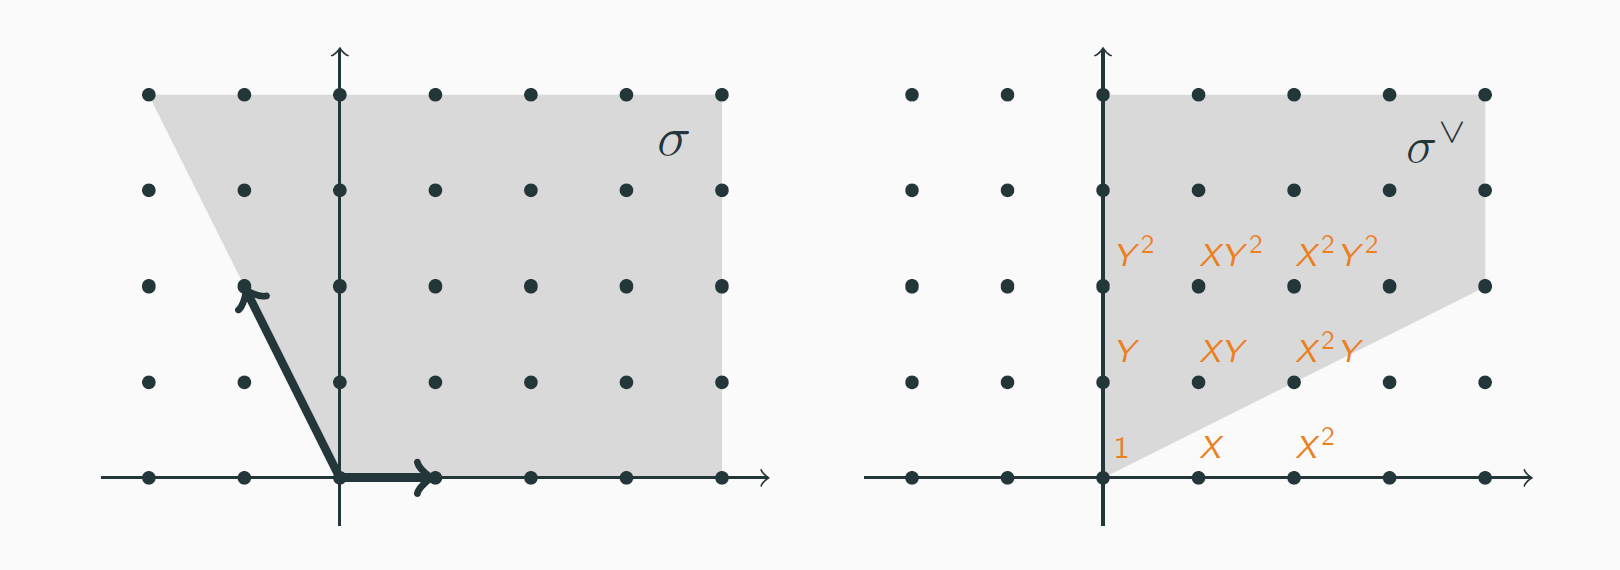
\includegraphics[width=0.8\textwidth]{cone_and_dual_with_monomials}}
\vspace{-0.2cm}
\begin{figure}[H]
    \centering
    \begin{tikzpicture}[scale=1.2]
        % Left diagram
        \begin{scope}[shift={(-2,0)}]
            % Shaded area
            \fill[gray!30] (0,0) -- (-1.05, 2.1) -- (2.1,2.1) -- (2.1,0) -- cycle;
            
            % Axes
            \draw[->] (-1.25,0) -- (2.25,0);
            \draw[->] (0,-0.25) -- (0,2.25);
            
            % Lattice points
            \foreach \x in {-1,-0.5,0,0.5,1,1.5,2}
                \foreach \y in {0,0.5,1,1.5,2}
                    \fill (\x,\y) circle (1pt);

            % Vectors
            %\draw[->, ultra thick] (0,0) -- (0.5,0);
            %\draw[->, ultra thick] (0,0) -- (-0.5,1);
            \node at (1.75, 1.75) {$\sigma$};
        \end{scope}

        % Right diagram
        \begin{scope}[shift={(2,0)}]
            % Shaded area
            \fill[gray!30] (0,0) -- (0,2.1) -- (2.1,2.1) -- (2.1, 1.05) -- cycle;
            
            % Axes
            \draw[->] (-1.25,0) -- (2.25,0);
            \draw[->] (0,-0.25) -- (0,2.25);
            
            % Lattice points
            \foreach \x in {-1,-0.5,0,0.5,1,1.5,2}
                \foreach \y in {0,0.5,1,1.5,2} {
                    \fill (\x,\y) circle (1pt);
                }
                
			  % Labels
			  \node[anchor=south west] at (0, 0) {\!\!\! \scriptsize \alert{$1$}};
			  
			  %\node[anchor=south] at (-0.5, 0) {\tiny \alert{$X^{-1}$}};
			  %\node[anchor=south] at (-0.5, 0.5) {\tiny \alert{$X^{-1} Y$}};
			  %\node[anchor=south] at (-0.5, 1) {\tiny \alert{$X^{-1} Y^2$}};
			  %\node[anchor=south] at (-0.5, 1.5) {\tiny \alert{$X^{-1} Y^3$}};
			
			  %\node[anchor=south ] at (-1, 0) {\, \scriptsize \alert{$r^{-2}$}};
			  %\node[anchor=south ] at (-1, 0.5) { \scriptsize \alert{$r^{-2} s$}};
			  %\node[anchor=south ] at (-1, 1) { \scriptsize \alert{$r^{-2} s^2$}};
  
			  \node[anchor=south ] at (-0.5, 0) {\scriptsize \alert{$r^{-1}$}};
			  \node[anchor=south ] at (-0.5, 0.5) { \scriptsize \alert{$r^{-1} s$}};
			  \node[anchor=south ] at (-0.5, 1) {\scriptsize \alert{$r^{-1} s^2$}};

			  \node[anchor=south west] at (0, 0.5) {\!\!\! \scriptsize \alert{$s$}};
			  \node[anchor=south west] at (0, 1) {\!\!\! \scriptsize \alert{$s^2$}};
			  %\node[anchor=south] at (0, 1.5) {\tiny \alert{$Y^3$}};
			  \node[anchor=south west] at (0.5, 0) {\!\!\!\! \scriptsize \alert{$r$}};
			  \node[anchor=south west] at (0.5, 0.5) {\!\!\!\! \scriptsize \alert{$r s$}};
			  \node[anchor=south west] at (0.5, 1) {\!\!\!\!  \scriptsize \alert{$r s^2$}};
			  %\node[anchor=south] at (0.5, 1.5) {\tiny \alert{$X Y^3$}};
			  \node[anchor=south west] at (1, 0) {\!\!\!\! \scriptsize \alert{$r^2$}};
			  \node[anchor=south west] at (1, 0.5) {\!\!\!\! \scriptsize \alert{$r^2 s$}};
			  \node[anchor=south west] at (1, 1) {\!\!\!\! \scriptsize \alert{$r^2 s^2$}};
			  %\node[anchor=south] at (1, 1.5) {\tiny \alert{$X^2 Y^3$}};

            % Vectors
            %\draw[->, ultra thick] (0,0) -- (0,0.5);
            %\draw[->, ultra thick] (0,0) -- (1,0.5);
            \node at (1.75, 1.75) {\small{$\sigma^\vee$}};
        \end{scope}
    \end{tikzpicture}
\end{figure}

\vspace{-0.3cm}

\pause
We create an algebra using the monomials in $\sigma^\vee$:
\begin{align*}
	\mathbb{C}[1, s, r^2 s, r s, s^2, rs^2, \ldots] &= \mathbb{C}[s, r^2 s, r s] \\
	&\cong \mathbb{C}[x, y, z]/(xy - z^2).
\end{align*}

\pause
The toric variety $U_\sigma$ is the set of solutions to $xy - z^2 = 0$ in $\mathbb{C}^3$:
$$xy = z^2.$$
\end{frame}

\begin{frame}
\frametitle{The definition of a toric variety}
\textbf{Fix}: cone $\sigma$, dual $\sigma^\vee$. 
The previous construction generalises.

\pause
We associate monomials $x_1^{i_1} \cdots x_n^{i_n}$ to integer points in $(\mathbb{R}^n)^*$.

\pause
We create an algebra using the monomials lying in $\sigma^\vee$, called $\mathbb{C}[S_\sigma]$.

\pause
$\mathbb{C}[S_\sigma]$ is finitely generated, so it's given by generators and relations:
$$\mathbb{C}[S_\sigma] = \mathbb{C}[y_1, \ldots, y_m]/(f_1, \ldots, f_s).$$

\pause
The \alert{toric variety} $U_\sigma$ is the subset of $\mathbb{C}^m$ defined by the equations
$$f_1(a_1, \ldots, a_m) = 0, \quad \ldots, \quad  f_s(a_1, \ldots, a_m) = 0.$$
\end{frame}


\begin{frame}
\frametitle{Cones detect singularities}

\onslide<2->{
\begin{theorem}
The toric variety $U_\sigma$ is non-singular if and only if $\sigma$ is generated by a subset of a basis for $\mathbb{Z}^n$.
\end{theorem}}


%\centerline{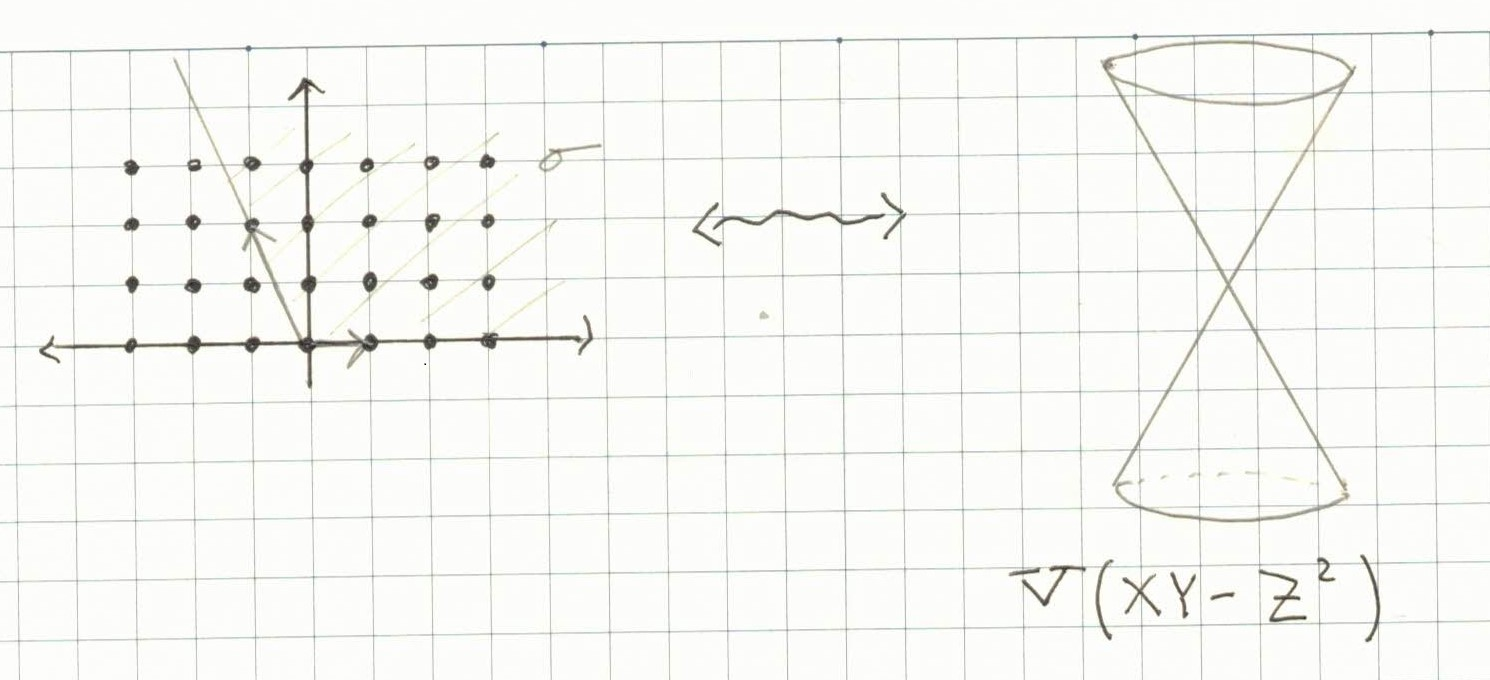
\includegraphics[width=\textwidth]{cone_and_variety}}
\onslide<3->{\begin{minipage}[t]{0.49\textwidth}
\centering
\begin{figure}
    
\includegraphics[width=0.7\linewidth]{orange_cone}
	\vspace{0cm}
    \caption*{$xy=z^2$}
\end{figure}
\end{minipage}}
\hfill
\onslide<3->{\begin{minipage}[t]{0.49\textwidth}
\centering
\vspace{0.5cm}
\begin{figure}
    \begin{tikzpicture}[scale=1.2]
        % Left diagram

            % Shaded area
            \fill[gray!30] (0,0) -- (-1.05, 2.1) -- (2.1,2.1) -- (2.1,0) -- cycle;
            
            % Axes
            \draw[->] (-1.25,0) -- (2.25,0);
            \draw[->] (0,-0.25) -- (0,2.25);
            
            % Lattice points
            \foreach \x in {-1,-0.5,0,0.5,1,1.5,2}
                \foreach \y in {0,0.5,1,1.5,2}
                    \fill (\x,\y) circle (1pt);

            % Vectors
            \onslide<3>{\draw[->, ultra thick] (0,0) -- (0.5,0);}
            \onslide<3>{\draw[->, ultra thick] (0,0) -- (-0.5,1);}

		% Lattice generated
		\onslide<4->{
            \draw[->, ultra thick, myorange] (0,0) -- (0.5,0);
            \draw[->, ultra thick, myorange] (0,0) -- (-0.5,1);
            \foreach \x in {-1,-0.5,0,0.5,1,1.5,2}
                \foreach \y in {0,1,2}
                    \fill[myorange] (\x,\y) circle (1.1pt);
		\foreach \x in {-1,-0.5,0,0.5,1}
			\draw[-, myorange] (\x - 0.1, 2 + 0.2) -- (\x + 1 + 0.1, 0 - 0.2);
		\draw[-, myorange] (-1 - 0.1, 1 + 0.2) -- (-1 + 0.5 + 0.1, 0 - 0.2);
		\draw[-, myorange] (1.5 - 0.1, 2 + 0.2) -- (1.5 + 0.5 + 0.1, 1 - 0.2);
		\draw[-, myorange] (-1.15, 0) -- (2.15, 0);
		\draw[-, myorange] (-1.15, 1) -- (2.15, 1);
		\draw[-, myorange] (-1.15, 2) -- (2.15, 2);
		}
        \end{tikzpicture}
\end{figure}
\end{minipage}}
\end{frame}

\begin{frame}
\frametitle{Torus quotients}


\end{frame}


\begin{frame}
\frametitle{References}
%\begin{adjustwidth}{-1.7em}{-1.7em}
\begin{enumerate}%[leftmargin=-1cm]
\item[]
Stephen Boyd and Lieven Vandenberghe,
\emph{Convex optimization},
Cambridge University Press, 2004.

\vspace{0.5cm}

\item[]
William Fulton,
\emph{Introduction to toric varieties},
Princeton University Press, 1993.

\vspace{0.5cm}

\item[]
Shigeru Mukai,
\emph{An introduction to invariants and moduli},
Cambridge University Press, 2003.

\vspace{0.5cm}

\item[]
Miles Reid,
\emph{Undergraduate algebraic geometry},
Cambridge Univeristy Press, 1988.
\end{enumerate}
%\end{adjustwidth}
\end{frame}
\end{document}